\documentclass[a4paper]{article}

\usepackage[czech]{babel} %https://github.com/michal-h21/biblatex-iso690
\usepackage[
   backend=biber      % if we want unicode 
  ,style=iso-numeric % or iso-numeric for numeric citation method          
  ,babel=other        % to support multiple languages in bibliography
  ,sortlocale=cs_CZ   % locale of main language, it is for sorting
  ,bibencoding=UTF8   % this is necessary only if bibliography file is in different encoding than main document
]{biblatex}

\usepackage[utf8]{inputenc}
\usepackage{fancyhdr}
\usepackage{amsmath}
\usepackage{amssymb}
\usepackage[left=2cm,right=2cm,top=2.5cm,bottom=2.5cm]{geometry}
\usepackage{graphicx}
\usepackage{pdfpages}
\usepackage{url}

\usepackage{siunitx}
\sisetup{locale = DE}  %, separate-uncertainty = true    kdybych chtel +/-

\usepackage{float}
\newfloat{graph}{htbp}{grp}
\floatname{graph}{Graf}
\newfloat{tabulka}{htbp}{tbl}
\floatname{tabulka}{Tabulka}

\renewcommand{\thefootnote}{\roman{footnote}}

\pagestyle{fancy}
\lhead{Praktikum II - (21) Studium hysterezních smyček feritů}
\rhead{Vladislav Wohlrath}
\author{Vladislav Wohlrath}

\bibliography{source}

\begin{document}

\begin{titlepage}
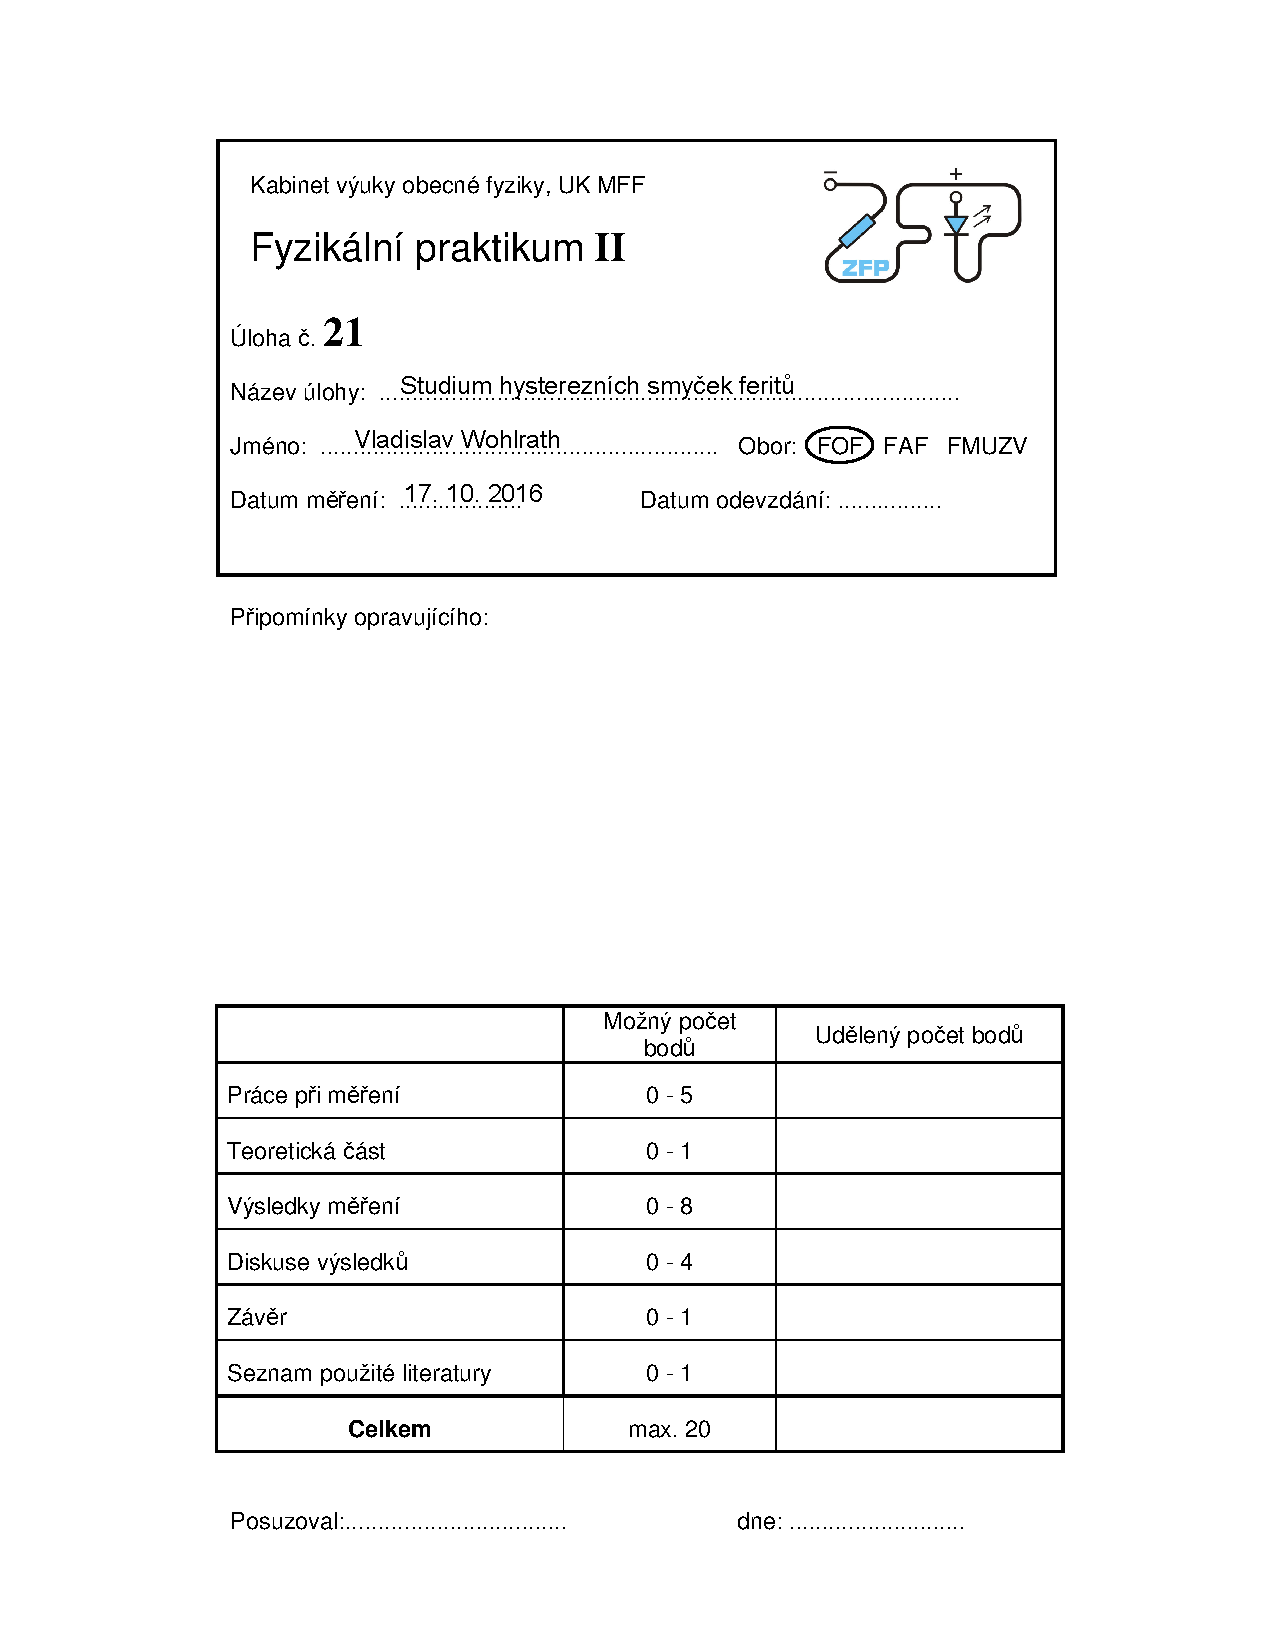
\includepdf[pages={1}]{./graficos/221-tit.pdf}
\end{titlepage}

\section*{Pracovní úkoly}
\begin{enumerate}
\item ÚKOLY
\end{enumerate}

%Teoretická část
\section*{Teoretická část}
Budeme sledovat hysterézní smyčky feritů.
Rozeznáváme tři základní typy hysterézních smyček --- úsečku, Rayleighův tvar a normální.

Používáme zapojení na obrázku \ref{o:schema}.

\begin{figure}[htbp]
\centering
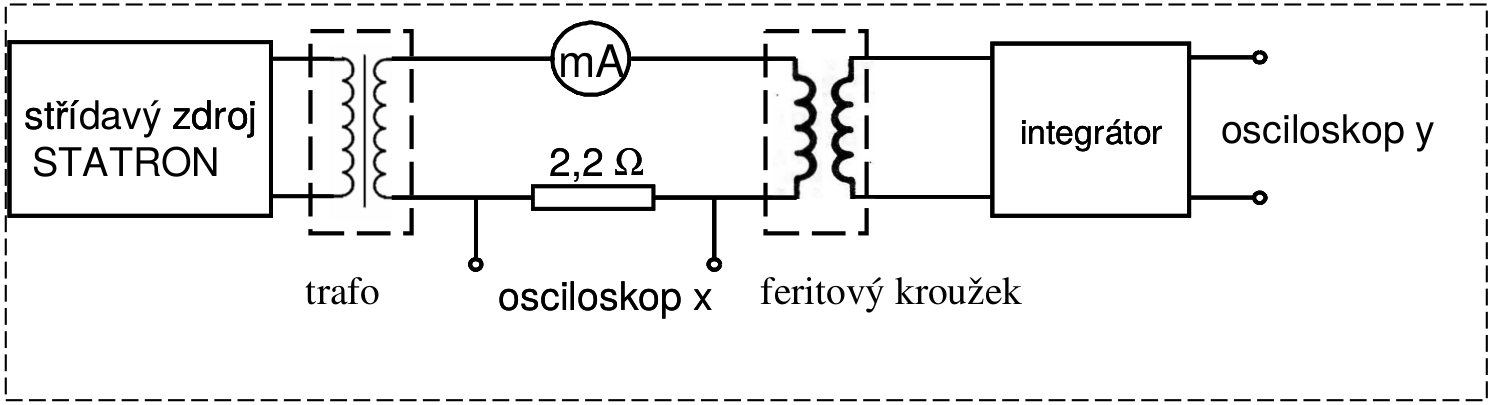
\includegraphics[width=\textwidth-2cm]{graficos/schema}
\caption{Zapojení pro pozorování hysterezních smyček}
\label{o:schema}
\end{figure}

Na miliampérmetru měříme efektivní hodnotu proudu $I_{ef}$, z něj určíme maximální intenzitu magnetického pole v kroužku
\begin{equation}
H_m=\frac{2 n_1 \sqrt{2} I_{ef}}{\pi (d_1+d_2)} \,,
\end{equation}
kde $n_1$ je počet závitů na primárním vinutí a $d_1$ a $d_2$ jsou vnitřní a vnější průměr kroužku.

Koercivní sílu $H_C$ určíme srovnáním s $H_m$ na stínítku osciloskopu.

Abychom mohli určit maximální magnetickou indukci $B_m$, okalibrujeme vertikální osu osciloskopu pomocí střídavého napětí známé velikosti.
Obvod zapojíme podle obrázku \ref{o:kalib} a pustíme do něj střídavé napětí o známé úhlové frekvenci $\omega$.

\begin{figure}[htbp]
\centering
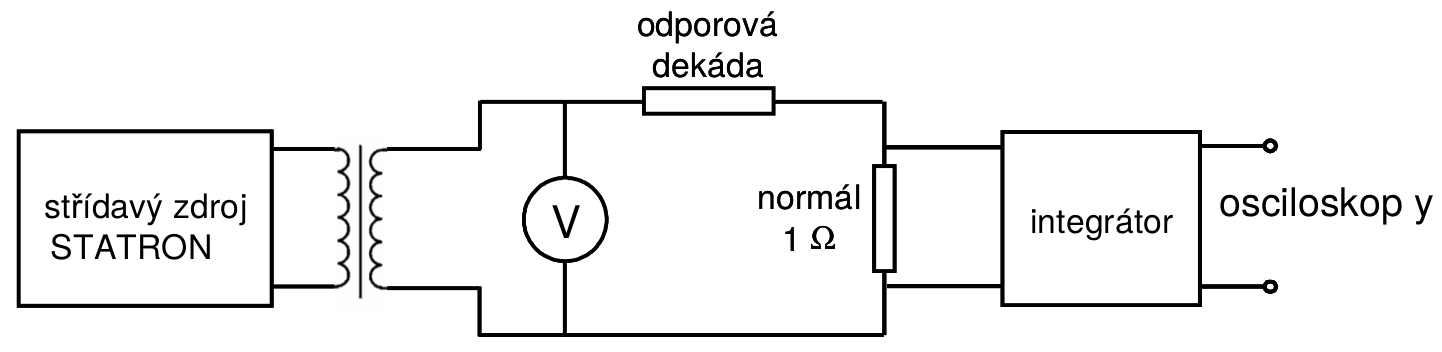
\includegraphics[width=\textwidth-2cm]{graficos/kalib}
\caption{Zapojení pro kalibraci vertikální osy}
\label{o:kalib}
\end{figure}

Na dekádě zvolíme odpor \SI{999}{\ohm}, takže efektivní hodnota napětí na normálu $U_{ef}$ bude rovna jedné tisícině udáje na voltmetru.
$B_m$ určíme jako \cite{skripta}
\begin{equation} \label{e:kalibrace}
B_m=\frac{U_{ef} \sqrt{2}}{\omega S n_2} \,,
\end{equation}
kde $n_2$ je počet závitů na sekundárním vinutí a $S$ je průřez kroužku
\begin{equation}
S=\frac{1}{2} (d_1-d_2) v \,,
\end{equation}
kde $v$ je výška kroužku.
Takto určíme jednu skutečnou hodnotu $B_m$ při plně rozvinuté hysterezní smyčce, ostatní určíme poměrně k ní.

%Podmínky a měřící přístroje
\section*{Podmínky a použité přístroje}

%Výsledky měření
\section*{Výsledky měření}

%Diskuze výsledků
\section*{Diskuze}
Použitý multimetr nebyl příliš přesný v porovnání s ostatními multimetry dostupnými v praktiku.
Zejména u třetího kroužku bylo použití tohoto multimetru krajně nevhodné a vysoce se podílelo na chybách naměřených hodnot.

Intenzity pole, při kterých se mění typ hysterezní smyčky, jsou skutečně jen přibližné.

Závislosti $H_C$ a $B_m$ na $H_m$ vyšly u všech kroužků podle očekávání.

U kroužku III se vyskytla jedna podezřelá hodnota $B_m$ ($H_C=\SI{3630}{\ampere\per\metre}$), kde závislost není monotónní (viz graf \ref{g:bm3}).
Ikdyž nemůžeme vyloučit pravdivost této hodnoty, nejpravděpodobněji se jedná o hrubou chybu při odečítání délky úsečky na stínítku, protože nemonotónnost této závislosti je jev, kterého bych si při měření jistě všimnul.

%Závěr
\section*{Závěr}
Změřili jsme závislost indukce $B_m$ a koercivní síly $H_C$ na intenzitě magnetického pole $H_m$ pro tři feritové kroužky (viz tabulka \ref{t:krouzky}).
Naměřené hodnoty jsou uvedeny v tabulce \ref{t:mereni} a zaneseny do grafů \ref{g:hc1} až \ref{g:bm3}.

Naměřené závislosti vyšly podle očekávání.


\printbibliography[title={Seznam použité literatury}]

\end{document}